\documentclass[landscape]{slides}
\usepackage[landscape, margin=2cm]{geometry}
\usepackage{color}
\usepackage{bm}
\usepackage{graphicx}
\usepackage{hyperref}
\usepackage{listings}
\definecolor{mygreen}{rgb}{0,0.6,0}
\definecolor{mymauve}{rgb}{0.58,0,0.82}
\lstset{ %
  backgroundcolor=\color{white},   % choose the background color; you must add \usepackage{color} or \usepackage{xcolor}
  basicstyle=\footnotesize,        % the size of the fonts that are used for the code
  commentstyle=\color{mygreen},    % comment style
  deletekeywords={...},            % if you want to delete keywords from the given language
  extendedchars=true,              % lets you use non-ASCII characters; for 8-bits encodings only, does not work with UTF-8
  frame=single,                    % adds a frame around the code
  keywordstyle=\color{blue},       % keyword style
  language=Python,                 % the language of the code
  rulecolor=\color{black},         % if not set, the frame-color may be changed on line-breaks within not-black text (e.g. comments (green here))
  showspaces=false,                % show spaces everywhere adding particular underscores; it overrides 'showstringspaces'
  stringstyle=\color{mymauve},     % string literal style
  title=\lstname                   % show the filename of files included with \lstinputlisting; also try caption instead of title
}
\hypersetup{
    colorlinks=true,
    urlcolor=blue
}

\graphicspath{ {./img/} {./charts/} }


\title{Factory Boy Fun}
\author{Adam Johnson - me@adamj.eu}
\date{9th September 2014}

\begin{document}

\maketitle

\begin{slide}
    \textcolor{blue}{\Large{What the problem?}}

    \begin{itemize}
        \item You've done this, right?
    \end{itemize}

    \begin{lstlisting}
# tests/test_something.py
class MyTests(TestCase):
    fixtures = ['basic.json']
    def setUp(self):
        self.user = User.objects.create(
            username='adam',
            first_name='Adam',
            last_name='Johnson',
            email='adam@example.com'
        )
        # ...
    # (and some tests, I hope!)
    \end{lstlisting}
\end{slide}


\begin{slide}
    \begin{lstlisting}
# tests/test_something.py
class MyTests(TestCase):
    fixtures = ['basic.json']
    def setUp(self):
        self.user = User.objects.create(
            username='adam',
            first_name='Adam',
            last_name='Johnson',
            email='adam@example.com'
        )
    \end{lstlisting}

    \textbf{Pain...}

    \begin{itemize}
        \item Test data in two places!
        \item A quirky json file that has to be maintained separately!
        \item I \emph{“just”} want a User but I have to give \emph{every} detail!
    \end{itemize}
\end{slide}


\begin{slide}
    \textcolor{blue}{\Large{Model-building can overtake testing}}

    \begin{itemize}
        \item Let's fix that... with a package ported from Ruby on Rails. (Trust me, it's gonna be okay!)
    \end{itemize}
\end{slide}


\begin{slide}
    \textcolor{blue}{\Large{Factories to the rescue!}}
    \begin{center}
        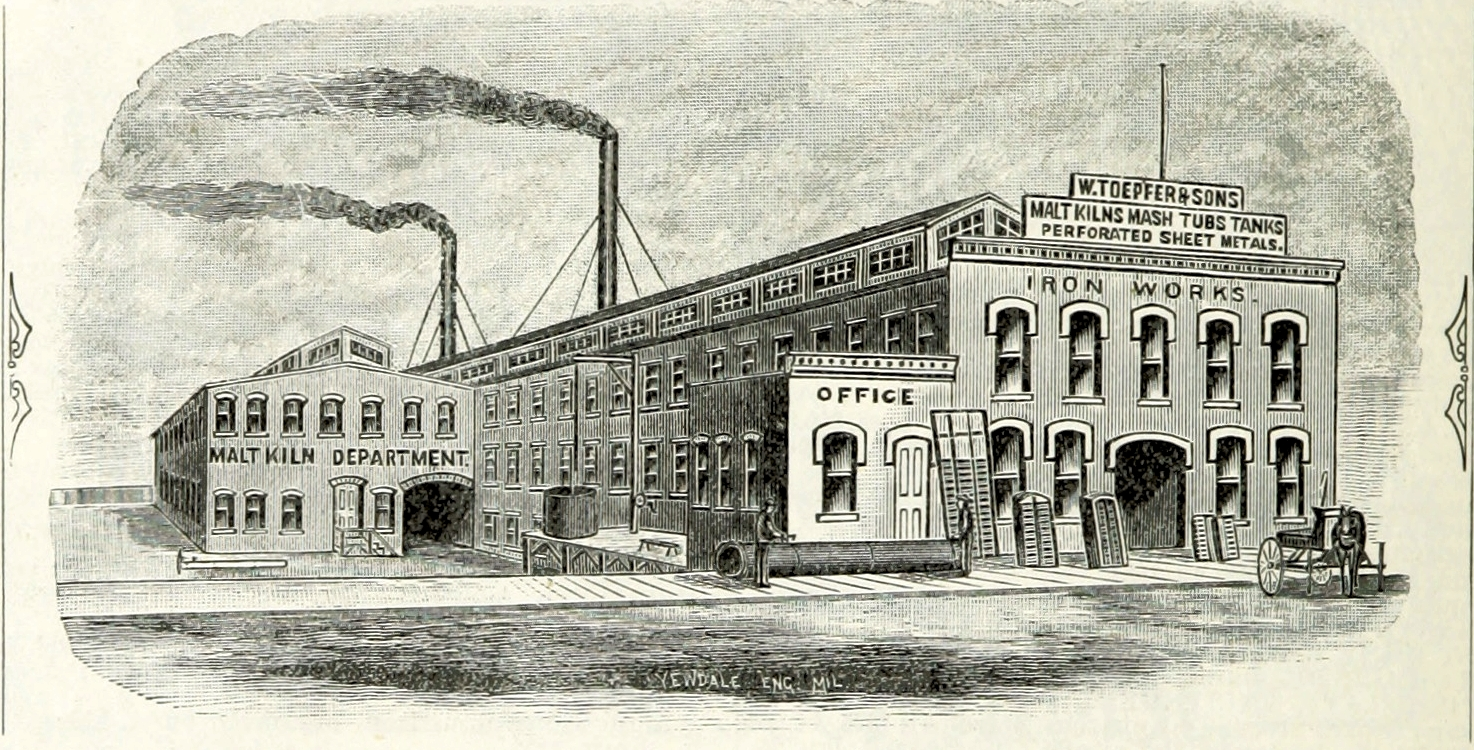
\includegraphics[height=12cm]{factory}
    \end{center}
\end{slide}


\begin{slide}
    \textcolor{blue}{\Large{Factory Boy}}

    \begin{itemize}
        \item ``A fixtures replacement based on thoughtbot's `factory\_girl'.''
        \item \url{http://factoryboy.readthedocs.org/en/latest/}
    \end{itemize}
\end{slide}



\begin{slide}
    \textcolor{blue}{\Large{Example factory}}

    \begin{itemize}
        \item Creates auth.User instances
    \end{itemize}
\end{slide}




\begin{slide}
    \begin{lstlisting}
class User(DjangoModelFactory):
    class Meta:
        model = 'auth.User'
        django_get_or_create = ('username',)

    first_name = 'Adam'
    last_name = 'Johnson'

    @lazy_attribute
    def username(self):
        return slugify(self.first_name + '.' +
                       self.last_name))

    @lazy_attribute
    def email(self):
        return self.username + "@example.com")

    @lazy_attribute
    def date_joined(self):
        return now() - timedelta(days=randint(5, 50))

    @lazy_attribute
    def last_login(self):
        return self.date_joined + dt.timedelta(days=4))
    \end{lstlisting}

\end{slide}


\begin{slide}
    \textcolor{blue}{\Large{Usage}}

    \begin{lstlisting}
class MyTests(TestCase):
    def setUp(self):
        # A single user, adam.johnson
        self.user = factories.User()

        # Another user, adam.smith
        self.user2 = factories.User(last_name='Smith')

        # A list of 10 users
        # (actually get_or_create -> 10 x adam.johnson)
        self.users = factories.User.create_batch(10)
    \end{lstlisting}

\end{slide}


\begin{slide}
    \textcolor{blue}{\Large{Adding fuzziness}}

    \begin{center}
        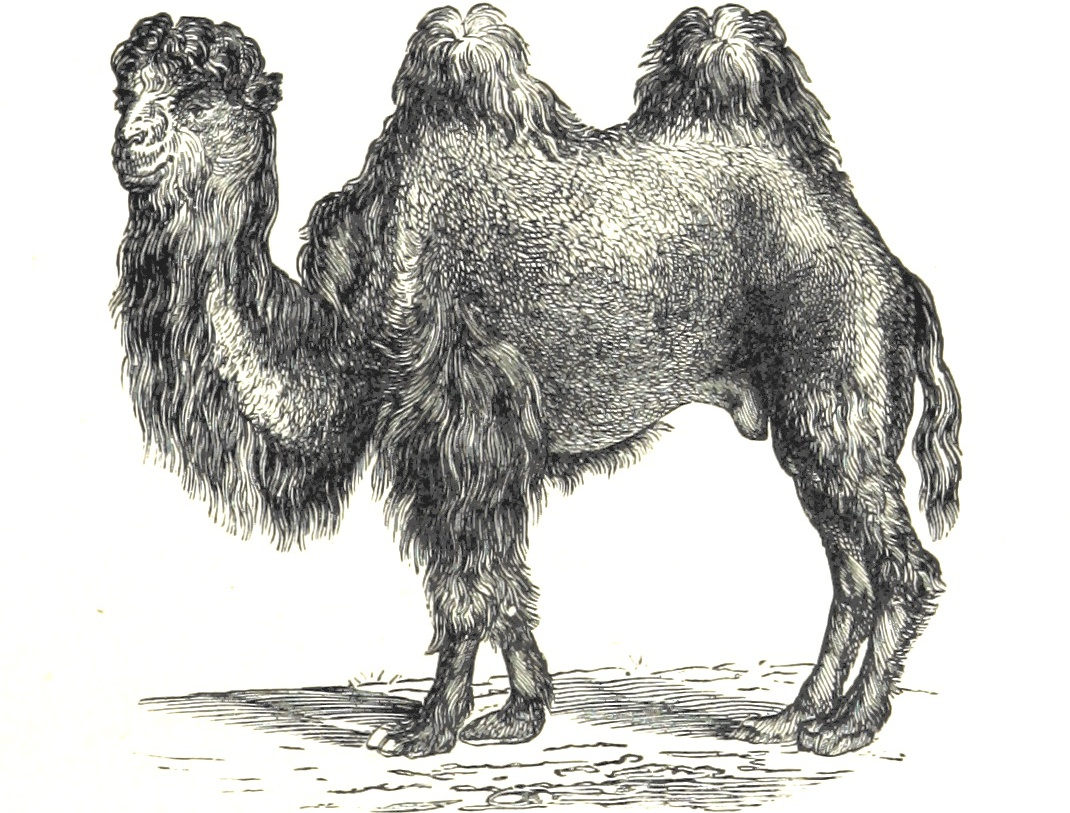
\includegraphics[height=12cm]{fuzzy}
    \end{center}
\end{slide}


\begin{slide}
    \textcolor{blue}{\Large{Adding fuzziness with faker}}

    \begin{itemize}
        \item A suite of functions for generating random test data
        \item \url{http://www.joke2k.net/faker/}
    \end{itemize}

    \begin{lstlisting}
import faker

# separate to a factory boy Factory
faker = faker.Factory.create()

class User(DjangoModelFactory):
    first_name = lazy(lambda o: faker.first_name())
    last_name = lazy(lambda o: faker.last_name())
    # ...
    \end{lstlisting}
\end{slide}


\begin{slide}
    \textcolor{blue}{\Large{Controlling the randomness}}

    \begin{itemize}
        \item Great for testing multiple paths
        \item But need control - if a test fails due to the randomness, how do we re-run it?
        \item For nose, install ``nose-randomize''. Prints random seed and lets you control it via ``--with-seed''.
    \end{itemize}
\end{slide}


\begin{slide}
    \textcolor{blue}{\Large{One-to-many relationships}}

    \begin{itemize}
        \item No built-in structure for navigating in particular
        \item But flexible ``post\_generation'' hook lets you add code
    \end{itemize}
\end{slide}


\begin{slide}
    \begin{lstlisting}
class Product(DjangoModelFactory):
    class Meta:
        model = 'app.Product'

    @lazy_attribute
    def name(self):
        return "Book by " + faker.name()

    @lazy_attribute
    def price(self):
        return Decimal(randint(5, 100))
    \end{lstlisting}

\end{slide}


\begin{slide}
    \begin{lstlisting}
class ProductGroup(DjangoModelFactory):
    class Meta:
        model = 'app.ProductGroup'

    @lazy_attribute
    def name(self):
        return "Products from " + faker.company()

    @post_generation
    def products(self, create, count, **kwargs):
        if count is None:
            count = 3

        make_product = getattr(Product,
            'create' if create else 'build')
        products = [make_product(group=self)
                    for i in range(count)]

        if not create:
            # Fiddle with django internals so
            # self.product_set.all() works with build()
            self._prefetched_objects_cache = \
                {'product': products}
    \end{lstlisting}
\end{slide}


\begin{slide}
    \textcolor{blue}{\Large{Usage}}

    \begin{lstlisting}
class MyTests(TestCase):
    def setUp(self):
        # A group of 10
        self.g1 = factories.ProductGroup(products=10)
    \end{lstlisting}
\end{slide}


\begin{slide}
    \textcolor{blue}{\Large{Problem solved?}}

    \begin{itemize}
        \item Helped us make terser, clearer tests
        \item Lower maintenance
        \item Useful also for populating local database with example data
    \end{itemize}
\end{slide}


\begin{slide}
    \textcolor{blue}{\Large{Thank you}}

    \begin{itemize}
        \item \url{me@adamj.eu}
    \end{itemize}
\end{slide}


\end{document}
